
\begin{frame}
  \frametitle{\kd trees}
  \framesubtitle{Nearest neighbor search}
  \begin{columns}[T]
    \begin{column}{.5\textwidth}
      \begin{block}{}%
        {\color{white} 1.\hspace{1mm} Compute orientation of point relative to hyperplane
          \\\vspace{0.4cm}
        
        2.\hspace{1mm} Recursively move down tree until leaf node\\\vspace{0.4cm}

        3.\hspace{1mm} Compare query point to all in leaf node, record smallest\\\vspace{0.4cm}
    
        4.\hspace{1mm} Upon return, if distance of point to hyperplane less than distance to current
          NN candidate, traverse other subtree}
      \end{block}
    \end{column}
    \begin{column}{.5\textwidth}
      \begin{block}{}
        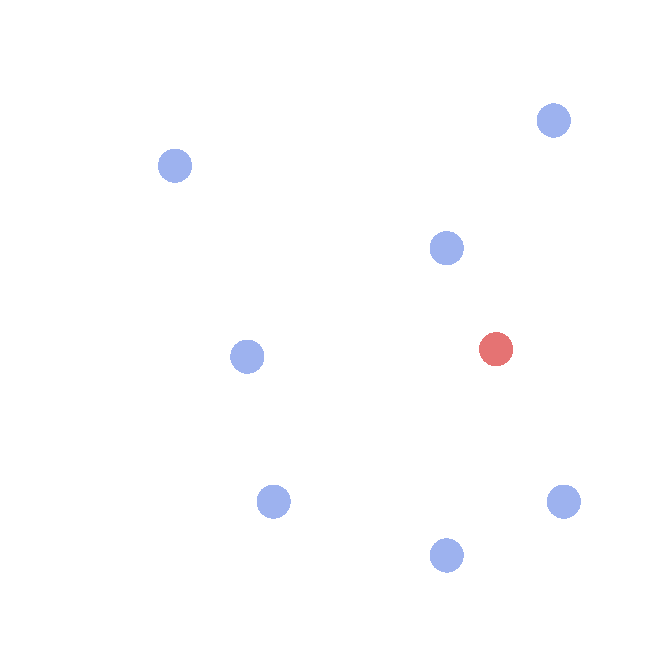
\includegraphics[width=0.85\textwidth]{nn_show1.pdf}
      \end{block}
    \end{column}
  \end{columns}
\end{frame}

\begin{frame}[noframenumbering]
  \frametitle{\kd trees}
  \framesubtitle{Nearest neighbor search}
  \begin{columns}[T]
    \begin{column}{.5\textwidth}
      \begin{block}{}%
        {\color{white} 

        {\color{graph-red}
        1.\hspace{1mm} Compute orientation of point relative to hyperplane}
          \\\vspace{0.4cm}
        
        2.\hspace{1mm} Recursively move down tree until leaf node\\\vspace{0.4cm}

        3.\hspace{1mm} Compare query point to all in leaf node, record smallest\\\vspace{0.4cm}
    
        4.\hspace{1mm} Upon return, if distance of point to hyperplane less than distance to current
          NN candidate, traverse other subtree}
      \end{block}
    \end{column}
    \begin{column}{.5\textwidth}
      \begin{block}{}
        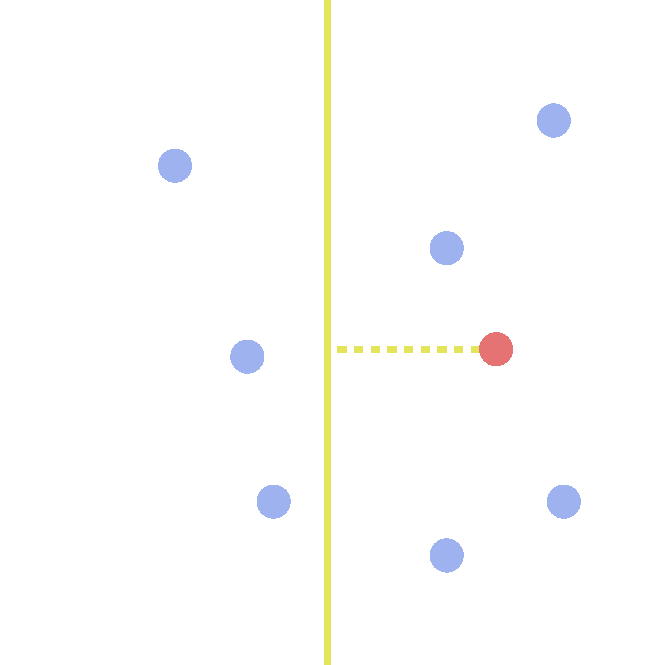
\includegraphics[width=0.85\textwidth]{nn_show2.pdf}
      \end{block}
    \end{column}
  \end{columns}
\end{frame}
\begin{frame}[noframenumbering]
  \frametitle{\kd trees}
  \framesubtitle{Nearest neighbor search}
  \begin{columns}[T]
    \begin{column}{.5\textwidth}
      \begin{block}{}%
        {\color{white} 1.\hspace{1mm} Compute orientation of point relative to hyperplane
          \\\vspace{0.4cm}

        {\color{graph-red}
        2.\hspace{1mm} Recursively move down tree until leaf node}\\\vspace{0.4cm}

        3.\hspace{1mm} Compare query point to all in leaf node, record smallest\\\vspace{0.4cm}
    
        4.\hspace{1mm} Upon return, if distance of point to hyperplane less than distance to current
          NN candidate, traverse other subtree}
      \end{block}
    \end{column}
    \begin{column}{.5\textwidth}
      \begin{block}{}
        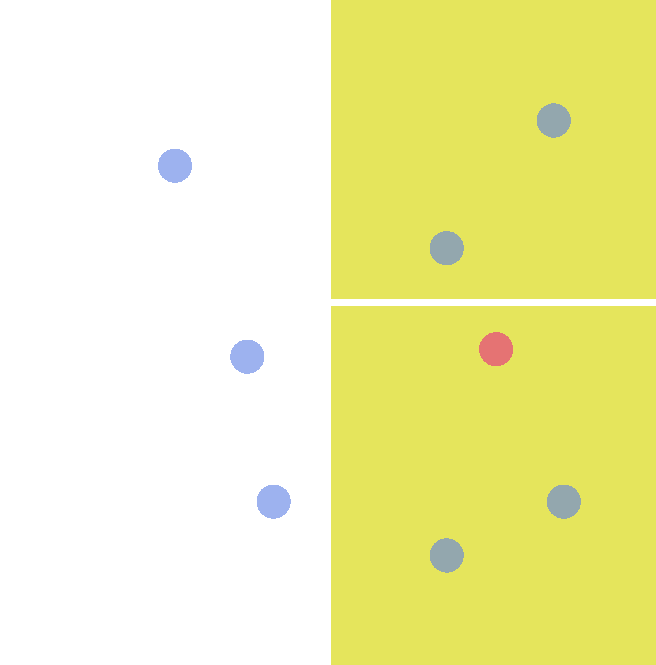
\includegraphics[width=0.85\textwidth]{nn_show3.pdf}
      \end{block}
    \end{column}
  \end{columns}
\end{frame}
\begin{frame}[noframenumbering]
  \frametitle{\kd trees}
  \framesubtitle{Nearest neighbor search}
  \begin{columns}[T]
    \begin{column}{.5\textwidth}
      \begin{block}{}%
        {\color{white} 
          
        {\color{graph-red}
        1.\hspace{1mm} Compute orientation of point relative to hyperplane}
          \\\vspace{0.4cm}
        
        2.\hspace{1mm} Recursively move down tree until leaf node\\\vspace{0.4cm}

        3.\hspace{1mm} Compare query point to all in leaf node, record smallest\\\vspace{0.4cm}
    
        4.\hspace{1mm} Upon return, if distance of point to hyperplane less than distance to current
          NN candidate, traverse other subtree}
      \end{block}
    \end{column}
    \begin{column}{.5\textwidth}
      \begin{block}{}
        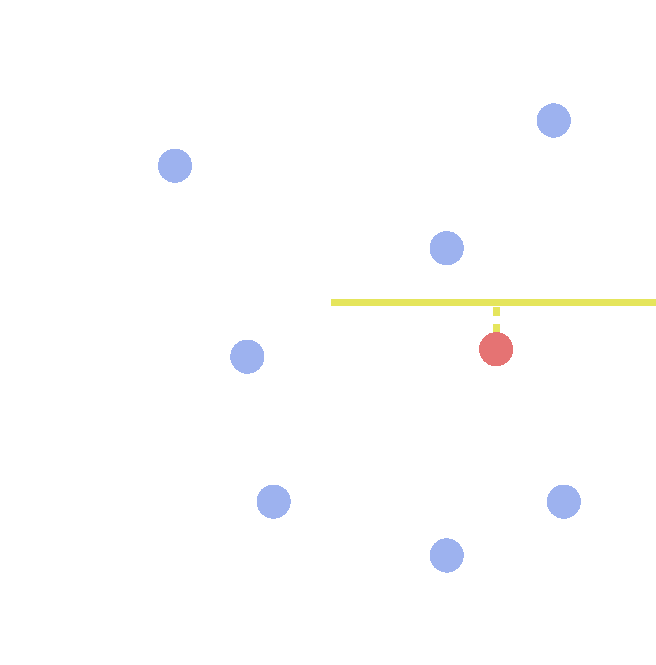
\includegraphics[width=0.85\textwidth]{nn_show4.pdf}
      \end{block}
    \end{column}
  \end{columns}
\end{frame}
\begin{frame}[noframenumbering]
  \frametitle{\kd trees}
  \framesubtitle{Nearest neighbor search}
  \begin{columns}[T]
    \begin{column}{.5\textwidth}
      \begin{block}{}%
        {\color{white} 1.\hspace{1mm} Compute orientation of point relative to hyperplane
          \\\vspace{0.4cm}

        {\color{graph-red}
        2.\hspace{1mm} Recursively move down tree until leaf node}\\\vspace{0.4cm}

        3.\hspace{1mm} Compare query point to all in leaf node, record smallest\\\vspace{0.4cm}
    
        4.\hspace{1mm} Upon return, if distance of point to hyperplane less than distance to current
          NN candidate, traverse other subtree}
      \end{block}
    \end{column}
    \begin{column}{.5\textwidth}
      \begin{block}{}
        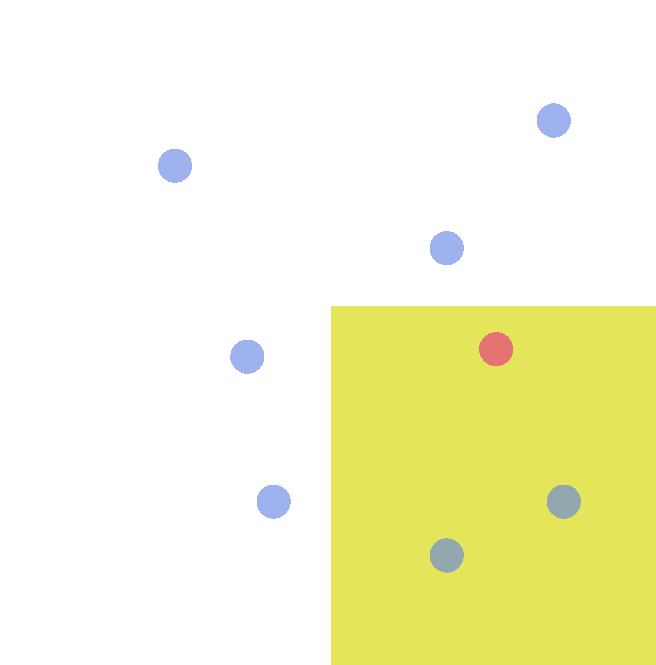
\includegraphics[width=0.85\textwidth]{nn_show5.pdf}
      \end{block}
    \end{column}
  \end{columns}
\end{frame}
\begin{frame}[noframenumbering]
  \frametitle{\kd trees}
  \framesubtitle{Nearest neighbor search}
  \begin{columns}[T]
    \begin{column}{.5\textwidth}
      \begin{block}{}%
        {\color{white} 1.\hspace{1mm} Compute orientation of point relative to hyperplane
          \\\vspace{0.4cm}
        
        2.\hspace{1mm} Recursively move down tree until leaf node\\\vspace{0.4cm}

        {\color{graph-red}
        3.\hspace{1mm} Compare query point to all in leaf node, record smallest}\\\vspace{0.4cm}
    
        4.\hspace{1mm} Upon return, if distance of point to hyperplane less than distance to current
          NN candidate, traverse other subtree}
      \end{block}
    \end{column}
    \begin{column}{.5\textwidth}
      \begin{block}{}
        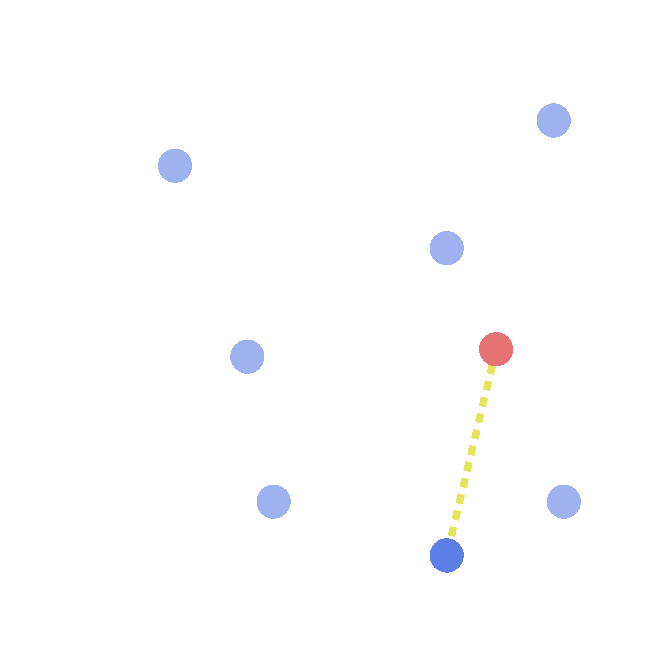
\includegraphics[width=0.85\textwidth]{nn_show6.pdf}
      \end{block}
    \end{column}
  \end{columns}
\end{frame}
\begin{frame}[noframenumbering]
  \frametitle{\kd trees}
  \framesubtitle{Nearest neighbor search}
  \begin{columns}[T]
    \begin{column}{.5\textwidth}
      \begin{block}{}%
        {\color{white} 1.\hspace{1mm} Compute orientation of point relative to hyperplane
          \\\vspace{0.4cm}
        
        2.\hspace{1mm} Recursively move down tree until leaf node\\\vspace{0.4cm}
        
        {\color{graph-red}
        3.\hspace{1mm} Compare query point to all in leaf node, record smallest}\\\vspace{0.4cm}
    
        4.\hspace{1mm} Upon return, if distance of point to hyperplane less than distance to current
          NN candidate, traverse other subtree}
      \end{block}
    \end{column}
    \begin{column}{.5\textwidth}
      \begin{block}{}
        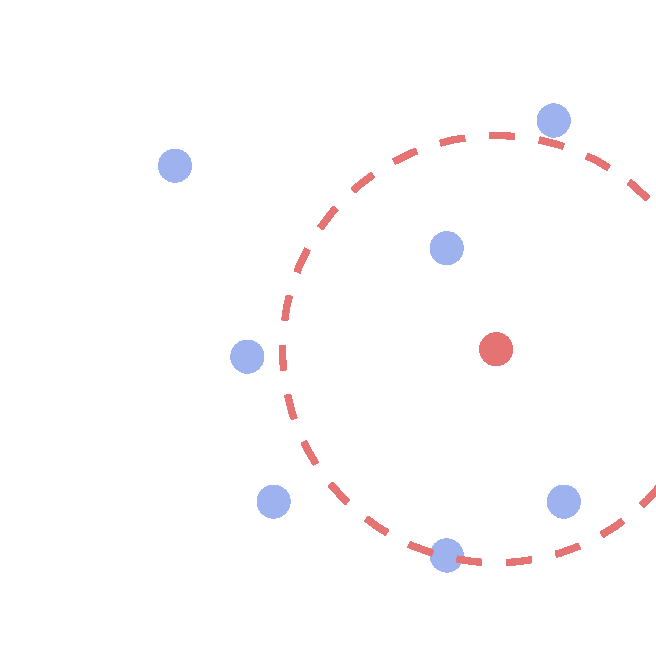
\includegraphics[width=0.85\textwidth]{nn_show7.pdf}
      \end{block}
    \end{column}
  \end{columns}
\end{frame}
\begin{frame}[noframenumbering]
  \frametitle{\kd trees}
  \framesubtitle{Nearest neighbor search}
  \begin{columns}[T]
    \begin{column}{.5\textwidth}
      \begin{block}{}%
        {\color{white} 1.\hspace{1mm} Compute orientation of point relative to hyperplane
          \\\vspace{0.4cm}
        
        2.\hspace{1mm} Recursively move down tree until leaf node\\\vspace{0.4cm}

        {\color{graph-red}
        3.\hspace{1mm} Compare query point to all in leaf node, record smallest}\\\vspace{0.4cm}
    
        4.\hspace{1mm} Upon return, if distance of point to hyperplane less than distance to current
          NN candidate, traverse other subtree}
      \end{block}
    \end{column}
    \begin{column}{.5\textwidth}
      \begin{block}{}
        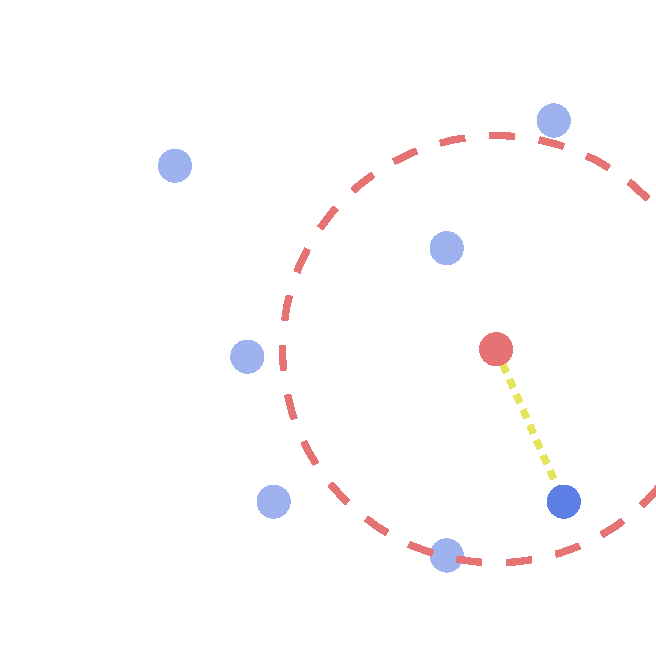
\includegraphics[width=0.85\textwidth]{nn_show8.pdf}
      \end{block}
    \end{column}
  \end{columns}
\end{frame}
\begin{frame}[noframenumbering]
  \frametitle{\kd trees}
  \framesubtitle{Nearest neighbor search}
  \begin{columns}[T]
    \begin{column}{.5\textwidth}
      \begin{block}{}%
        {\color{white} 1.\hspace{1mm} Compute orientation of point relative to hyperplane
          \\\vspace{0.4cm}
        
        2.\hspace{1mm} Recursively move down tree until leaf node\\\vspace{0.4cm}

        {\color{graph-red}
        3.\hspace{1mm} Compare query point to all in leaf node, record smallest}\\\vspace{0.4cm}
    
        4.\hspace{1mm} Upon return, if distance of point to hyperplane less than distance to current
          NN candidate, traverse other subtree}
      \end{block}
    \end{column}
    \begin{column}{.5\textwidth}
      \begin{block}{}
        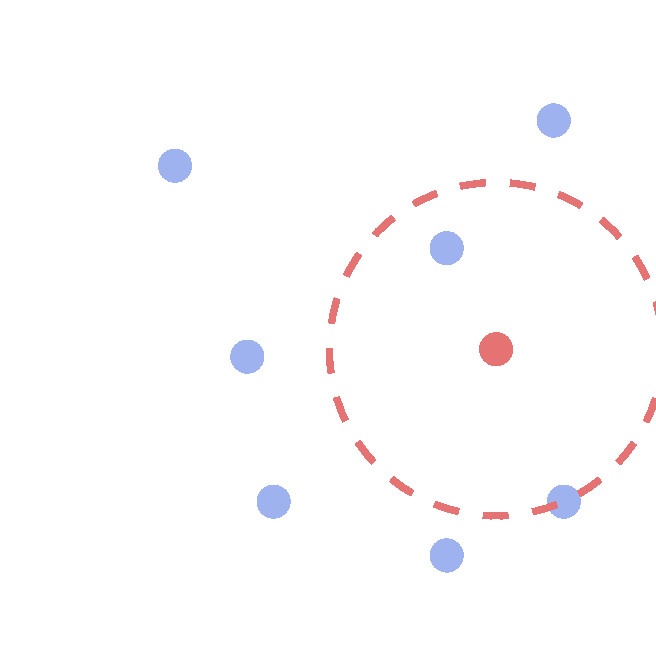
\includegraphics[width=0.85\textwidth]{nn_show9.pdf}
      \end{block}
    \end{column}
  \end{columns}
\end{frame}
\begin{frame}[noframenumbering]
  \frametitle{\kd trees}
  \framesubtitle{Nearest neighbor search}
  \begin{columns}[T]
    \begin{column}{.5\textwidth}
      \begin{block}{}%
        {\color{white} 1.\hspace{1mm} Compute orientation of point relative to hyperplane
          \\\vspace{0.4cm}
        
        2.\hspace{1mm} Recursively move down tree until leaf node\\\vspace{0.4cm}

        3.\hspace{1mm} Compare query point to all in leaf node, record smallest\\\vspace{0.4cm}
    
        {\color{graph-red}
        4.\hspace{1mm} Upon return, if distance of point to hyperplane less than distance to current
      NN candidate, traverse other subtree}}
      \end{block}
    \end{column}
    \begin{column}{.5\textwidth}
      \begin{block}{}
        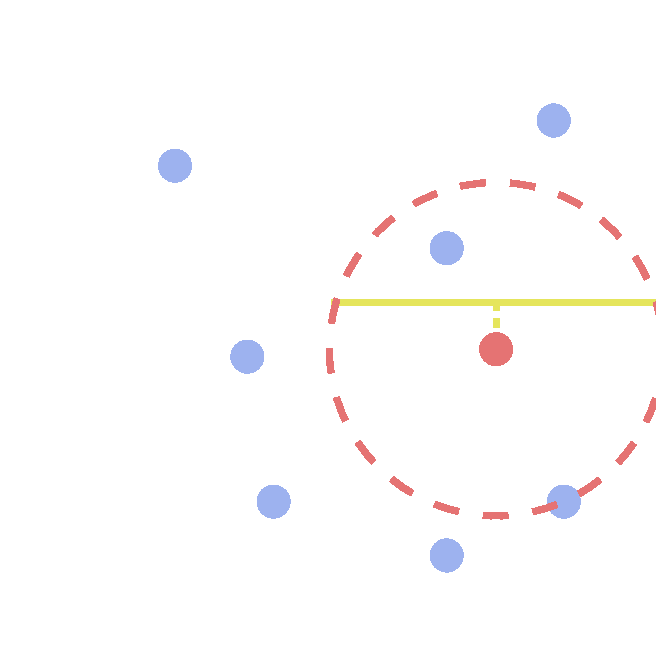
\includegraphics[width=0.85\textwidth]{nn_show10.pdf}
      \end{block}
    \end{column}
  \end{columns}
\end{frame}

\begin{frame}[noframenumbering]
  \frametitle{\kd trees}
  \framesubtitle{Nearest neighbor search}
  \begin{columns}[T]
    \begin{column}{.5\textwidth}
      \begin{block}{}%
        {\color{white} 1.\hspace{1mm} Compute orientation of point relative to hyperplane
          \\\vspace{0.4cm}
        
        2.\hspace{1mm} Recursively move down tree until leaf node\\\vspace{0.4cm}

        3.\hspace{1mm} Compare query point to all in leaf node, record smallest\\\vspace{0.4cm}
    
        {\color{graph-red}
        4.\hspace{1mm} Upon return, if distance of point to hyperplane less than distance to current
        NN candidate, traverse other subtree}}
      \end{block}
    \end{column}
    \begin{column}{.5\textwidth}
      \begin{block}{}
        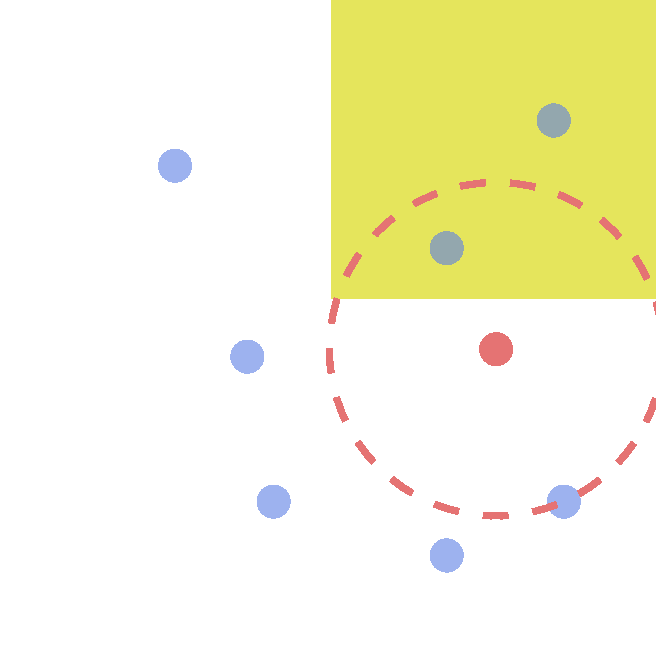
\includegraphics[width=0.85\textwidth]{nn_show11.pdf}
      \end{block}
    \end{column}
  \end{columns}
\end{frame}
\begin{frame}[noframenumbering]
  \frametitle{\kd trees}
  \framesubtitle{Nearest neighbor search}
  \begin{columns}[T]
    \begin{column}{.5\textwidth}
      \begin{block}{}%
        {\color{white} 1.\hspace{1mm} Compute orientation of point relative to hyperplane
          \\\vspace{0.4cm}
        
        2.\hspace{1mm} Recursively move down tree until leaf node\\\vspace{0.4cm}

        {\color{graph-red}
        3.\hspace{1mm} Compare query point to all in leaf node, record smallest}\\\vspace{0.4cm}
    
        4.\hspace{1mm} Upon return, if distance of point to hyperplane less than distance to current
          NN candidate, traverse other subtree}
      \end{block}
    \end{column}
    \begin{column}{.5\textwidth}
      \begin{block}{}
        \includegraphics[width=0.85\textwidth]{nn_show12.pdf}
      \end{block}
    \end{column}
  \end{columns}
\end{frame}
\begin{frame}[noframenumbering]
  \frametitle{\kd trees}
  \framesubtitle{Nearest neighbor search}
  \begin{columns}[T]
    \begin{column}{.5\textwidth}
      \begin{block}{}%
        {\color{white} 1.\hspace{1mm} Compute orientation of point relative to hyperplane
          \\\vspace{0.4cm}
        
        2.\hspace{1mm} Recursively move down tree until leaf node\\\vspace{0.4cm}

        {\color{graph-red}
        3.\hspace{1mm} Compare query point to all in leaf node, record smallest}\\\vspace{0.4cm}
    
        4.\hspace{1mm} Upon return, if distance of point to hyperplane less than distance to current
          NN candidate, traverse other subtree}
      \end{block}
    \end{column}
    \begin{column}{.5\textwidth}
      \begin{block}{}
        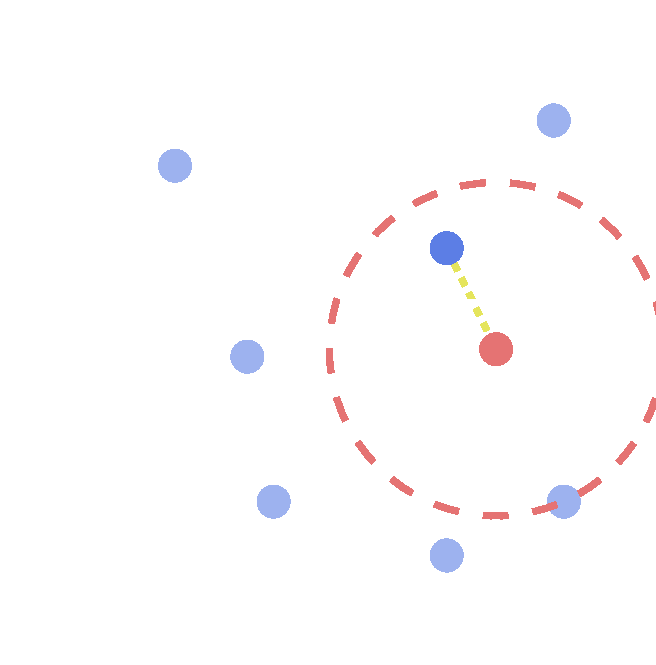
\includegraphics[width=0.85\textwidth]{nn_show13.pdf}
      \end{block}
    \end{column}
  \end{columns}
\end{frame}
\begin{frame}[noframenumbering]
  \frametitle{\kd trees}
  \framesubtitle{Nearest neighbor search}
  \begin{columns}[T]
    \begin{column}{.5\textwidth}
      \begin{block}{}%
        {\color{white} 1.\hspace{1mm} Compute orientation of point relative to hyperplane
          \\\vspace{0.4cm}
        
        2.\hspace{1mm} Recursively move down tree until leaf node\\\vspace{0.4cm}

        {\color{graph-red}
        3.\hspace{1mm} Compare query point to all in leaf node, record smallest}\\\vspace{0.4cm}
    
        4.\hspace{1mm} Upon return, if distance of point to hyperplane less than distance to current
          NN candidate, traverse other subtree}
      \end{block}
    \end{column}
    \begin{column}{.5\textwidth}
      \begin{block}{}
        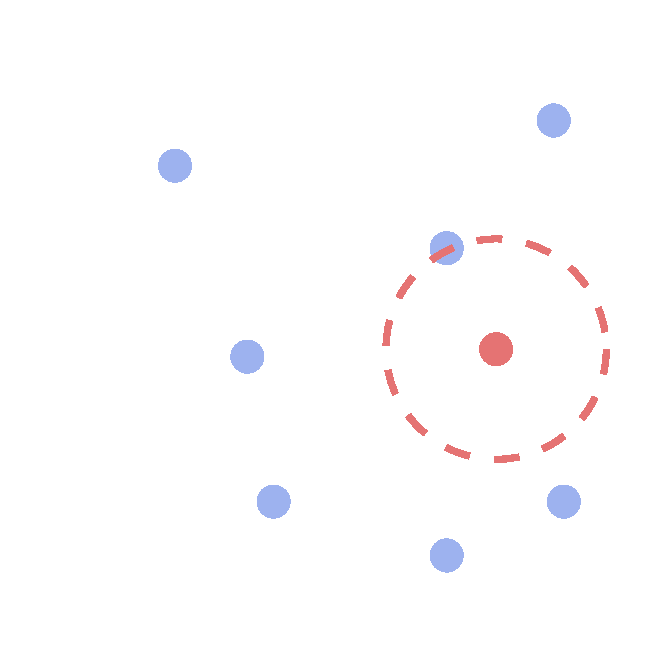
\includegraphics[width=0.85\textwidth]{nn_show14.pdf}
      \end{block}
    \end{column}
  \end{columns}
\end{frame}
\begin{frame}[noframenumbering]
  \frametitle{\kd trees}
  \framesubtitle{Nearest neighbor search}
  \begin{columns}[T]
    \begin{column}{.5\textwidth}
      \begin{block}{}%
        {\color{white} 1.\hspace{1mm} Compute orientation of point relative to hyperplane
          \\\vspace{0.4cm}
        
        2.\hspace{1mm} Recursively move down tree until leaf node\\\vspace{0.4cm}

        3.\hspace{1mm} Compare query point to all in leaf node, record smallest\\\vspace{0.4cm}
    
        {\color{graph-red}
        4.\hspace{1mm} Upon return, if distance of point to hyperplane less than distance to current
    NN candidate, traverse other subtree}}
      \end{block}
    \end{column}
    \begin{column}{.5\textwidth}
      \begin{block}{}
        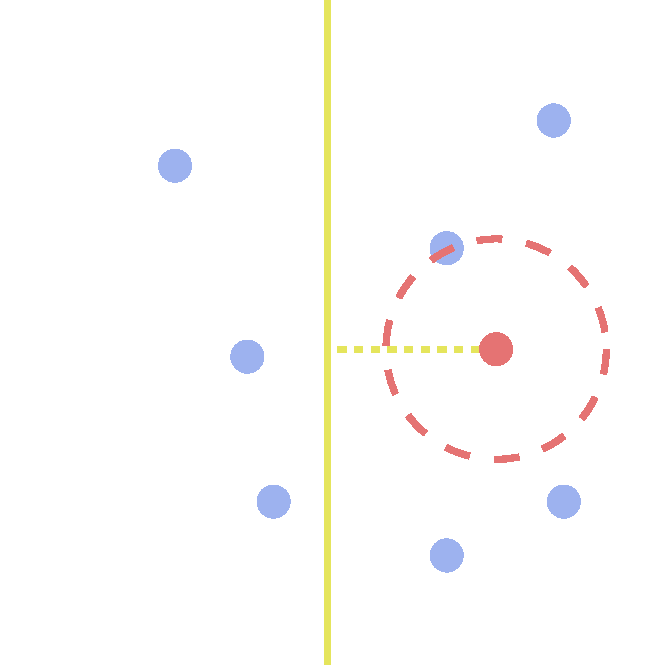
\includegraphics[width=0.85\textwidth]{nn_show15.pdf}
      \end{block}
    \end{column}
  \end{columns}
\end{frame}
\begin{frame}[noframenumbering]
  \frametitle{\kd trees}
  \framesubtitle{Nearest neighbor search}
  \begin{columns}[T]
    \begin{column}{.5\textwidth}
      \begin{block}{}%
        {\color{white} 1.\hspace{1mm} Compute orientation of point relative to hyperplane
          \\\vspace{0.4cm}
        
        2.\hspace{1mm} Recursively move down tree until leaf node\\\vspace{0.4cm}

        3.\hspace{1mm} Compare query point to all in leaf node, record smallest\\\vspace{0.4cm}
    
        4.\hspace{1mm} Upon return, if distance of point to hyperplane less than distance to current
          NN candidate, traverse other subtree}
      \end{block}
    \end{column}
    \begin{column}{.5\textwidth}
      \begin{block}{}
        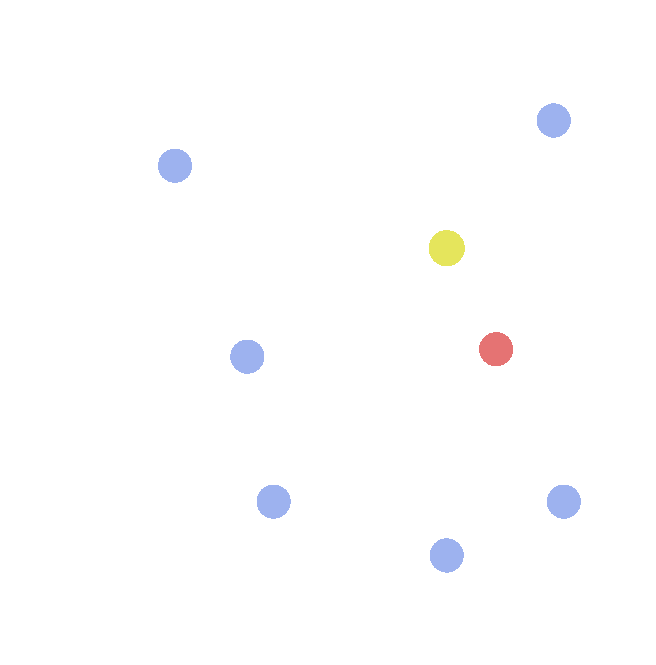
\includegraphics[width=0.85\textwidth]{nn_show16.pdf}
      \end{block}
    \end{column}
  \end{columns}
\end{frame}
